% File: Car2D.tex
% Author: Adam Leeper
%------------------------------------------------------------------------------
\providecommand{\isolatedBuild}[1]{#1}% Fallback definition to build normally.
\isolatedBuild{
  \documentclass[11pt,letterpaper]{book}
  %\documentclass[11pt,letterpaper]{book}

% aleeper: I think these are needed for Paul's macros?
\usepackage{epsfig}
\usepackage{epstopdf}

%\makeatletter
%\typeout{The import path is \import@path}
%\makeatother

\usepackage{import}

\subimport{./}{packagesMitiguy.sty}
\subimport{./}{macrosMitiguy.tex}
\subimport{./}{PageStylesMitiguy.tex}
\subimport{./}{macrosLeeper.tex}
   % Found via TEXINPUTS environment variable.
  \isolatedBuildHeader{2D Rigid Body Equations of Motion}
                      {Vehicle Equations of Motion}
}
%%%
%%%
%%%
The figure below shows a top-view of a vehicle B with mass $m$
and moment of inertia $\iscalarzz{B/\cm{B}} = I$, skidding on a flat
road \basis{N} (regarded as a Newtonian reference frame).
Right-handed orthogonal unit vectors \uvecxyz{b} are fixed in \basis{B} as
shown.
Using scalar variables $v_x$, $v_y$, and $\omega$, the vehicle's motion in
\basis{N} can be characterized by the velocity of \cm{B} (\basis{B}'s mass
center) and \basis{B}'s angular velocity as
%where  are variables and
\\[0.5pc]
\begin{tabular}{@{\hspace{1cm}}c@{\hspace{1cm}}c}
  $\vel{\cm{B}}{N} = v_x~\uvecx{b} + v_y~\uvecy{b}$
  &
  $\angvel{B}{N} = \omega~\uvecz{b}$
\end{tabular}
%
\\[0.5pc]
The \textbf{resultant} of all forces on the vehicle (e.g. forces due to tires,
road, aerodynamics, \textit{etc.}) and the moment of those forces about \cm{B}
can be written as
%
\\[0.5pc]
\begin{tabular}{@{\hspace{1cm}}c@{\hspace{1cm}}c}
  $\force{B} = F_x~\uvecx{b} + F_y~\uvecy{b}$
  &
  $\moment{B/\cm{B}} = T_z~\uvecz{b}$
\end{tabular}
%
\begin{enumerate}
  \item \textbf{Show} that
    $\accel{\cm{B}}{N} = (\vxdot - \omega \vy)\uvecx{b}
                       + (\vydot + \omega \vy)\uvecy{b}$
  \item Obtain a set of 3 scalar differential equations
    (for $\vxdot$, $\vydot$, $\omegadot$) that could be used to predict
    (or simulate) the vehicle's motion.\footnote{These equations could be a
    first step toward designing a steering and/or braking stability control
    system, or for simulating the motion of the vehicle in 2D racing game,
    etc.} First complete the roadmap table, then follow the map!
    \\[0.0pc]\textbf{Hint:} Don't introduce an angle. Just don't.
    \\[1.0pc]
    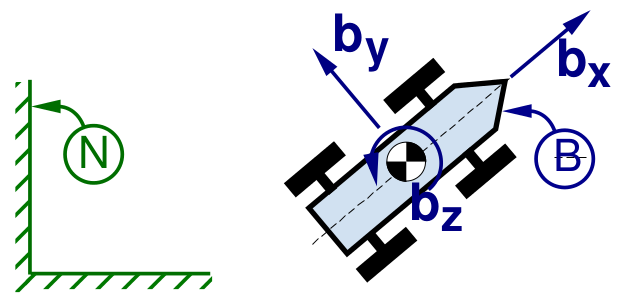
\includegraphics[width=5cm]{car.png}
    \\[1.0pc]
\end{enumerate}
%
\isolatedBuildFooter
